%% bare_conf.tex
%% V1.4b
%% 2015/08/26
%% by Michael Shell
%% See:
%% http://www.michaelshell.org/
%% for current contact information.
%%
%% This is a skeleton file demonstrating the use of IEEEtran.cls
%% (requires IEEEtran.cls version 1.8b or later) with an IEEE
%% conference paper.
%%
%% Support sites:
%% http://www.michaelshell.org/tex/ieeetran/
%% http://www.ctan.org/pkg/ieeetran
%% and
%% http://www.ieee.org/

%%*************************************************************************
%% Legal Notice:
%% This code is offered as-is without any warranty either expressed or
%% implied; without even the implied warranty of MERCHANTABILITY or
%% FITNESS FOR A PARTICULAR PURPOSE! 
%% User assumes all risk.
%% In no event shall the IEEE or any contributor to this code be liable for
%% any damages or losses, including, but not limited to, incidental,
%% consequential, or any other damages, resulting from the use or misuse
%% of any information contained here.
%%
%% All comments are the opinions of their respective authors and are not
%% necessarily endorsed by the IEEE.
%%
%% This work is distributed under the LaTeX Project Public License (LPPL)
%% ( http://www.latex-project.org/ ) version 1.3, and may be freely used,
%% distributed and modified. A copy of the LPPL, version 1.3, is included
%% in the base LaTeX documentation of all distributions of LaTeX released
%% 2003/12/01 or later.
%% Retain all contribution notices and credits.
%% ** Modified files should be clearly indicated as such, including  **
%% ** renaming them and changing author support contact information. **
%%*************************************************************************

\let\emph\textit
% *** Authors should verify (and, if needed, correct) their LaTeX system  ***
% *** with the testflow diagnostic prior to trusting their LaTeX platform ***
% *** with production work. The IEEE's font choices and paper sizes can   ***
% *** trigger bugs that do not appear when using other class files.       ***                          ***
% The testflow support page is at:
% http://www.michaelshell.org/tex/testflow/
\documentclass[conference,a4paper]{IEEEtran}
% Some Computer Society conferences also require the compsoc mode option,
% but others use the standard conference format.
%
% If IEEEtran.cls has not been installed into the LaTeX system files,
% manually specify the path to it like:
% \documentclass[conference]{../sty/IEEEtran}

\usepackage{amsmath}
\usepackage{amsmath,bm}
\usepackage{amssymb}
\usepackage{multicol}
\usepackage{graphicx}
\usepackage{epstopdf}
\usepackage{booktabs}
\usepackage{color}
\usepackage{psfrag}
\usepackage{cleveref}
\usepackage{cite}
%\usepackage{hyperref}
\usepackage{acronym}
\usepackage{arydshln}
%\usepackage{subfig}
\usepackage{stfloats}
\usepackage{subfigure}
\usepackage{caption}
\usepackage{setspace}
\usepackage{amssymb}
\usepackage{latexsym}


\captionsetup{font={small}}

\pagestyle{empty}



\newcommand{\Rx} {\mathrm{Rx}}
\newcommand{\Tx} {\mathrm{Tx}}
\newcommand{\iRe} {\mathrm{Re}}
\newcommand{\iIm} {\mathrm{Im}}
\newcommand{\iT} {\mathrm{T}}    % Generally for Transpose
\newcommand{\iH} {\mathrm{H}}    % Generally for Hermite Transpose
\newcommand{\iR} {\mathrm{R}}
\newcommand{\iI} {\mathrm{I}}
\newcommand{\iS} {\mathrm{S}}
\newcommand{\idt} {\mathrm{d}t}   % for integral dt
\newcommand{\idf} {\mathrm{d}f}   % for integral dt
\newcommand{\iRM}[1] {\mathrm{#1}}
\newcommand{\iNa} {N_\mathrm{a}}
\newcommand{\iNb} {N_\mathrm{b}}
\newcommand{\iTob} {T_\mathrm{ob}}



\DeclareMathOperator*{\argmin}{arg~min}
\DeclareMathOperator*{\argmax}{arg~max}
\DeclareMathOperator*{\diag}{diag}
\DeclareMathOperator*{\blkdiag}{blkdiag}
\DeclareMathOperator*{\trace}{tr}

%-------------RBPF----------------
\newcommand{\Cop} {\mathrm{c}}    % cooperation
\newcommand{\Agn} {\mathrm{a}}    % agent
\newcommand{\Anc} {\mathrm{b}}    % anchor
\newcommand{\LOS} {\mathrm{L}}    % anchor
\newcommand{\NLOS} {\mathrm{NL}}    % anchor
%-------------RBPF----------------


%\usepackage[ngerman]{babel}
%\usepackage{sansmath}
%\sansmath
%\usepackage[utf8]{inputenc}
%\usepackage[T1]{fontenc}
%\usepackage{upgreek}
%\usepackage{amsmath, amssymb}

%% =========== Euler ==========
%\DeclareMathAlphabet{\matheur}{U}{eur}{m}{n}
%\SetMathAlphabet{\matheur}{bold}{U}{eur}{b}{n}
%\DeclareRobustCommand{\msf}[1]{%
%  \ifcat\noexpand#1\relax\msfgreek{#1}\else\matheur{#1}\fi%for math sans serif (Euler)
%}
%% =========================
%
%% ==== Computer Modern Sans Serif ====
\DeclareMathAlphabet{\mathsfbr}{OT1}{cmss}{m}{n}%for math sans serif (cmss)
\SetMathAlphabet{\mathsfbr}{bold}{OT1}{cmss}{bx}{n}%for math sans serif (cmss)
\DeclareRobustCommand{\msf}[1]{%
	\ifcat\noexpand#1\relax\msfgreek{#1}\else\mathsfbr{#1}\fi%for math sans serif (cmss)
}
%% =========================

% ==== Computer Modern Bright ====
%% Part 1: This is necessary to fix a bug in the .fd file of the font!!!
%\DeclareFontFamily{OT1}{cmbr}{\hyphenchar\font45 }
%\DeclareFontShape{OT1}{cmbr}{m}{n}{%
%  <-9>cmbr8
%  <9-10>cmbr9
%  <10-17>cmbr10
%  <17->cmbr17
%}{}
%\DeclareFontShape{OT1}{cmbr}{m}{sl}{%
%  <-9>cmbrsl8
%  <9-10>cmbrsl9
%  <10-17>cmbrsl10
%  <17->cmbrsl17
%}{}
%\DeclareFontShape{OT1}{cmbr}{m}{it}{%
%  <->ssub*cmbr/m/sl
%}{}
%\DeclareFontShape{OT1}{cmbr}{b}{n}{%
%  <->ssub*cmbr/bx/n
%}{}
%\DeclareFontShape{OT1}{cmbr}{bx}{n}{%
%  <->cmbrbx10
%}{}
%% Part 2
%\DeclareMathAlphabet{\mathsfbr}{OT1}{cmbr}{m}{n}%for math sans serif bright (cmbr)
%\SetMathAlphabet{\mathsfbr}{bold}{OT1}{cmbr}{b}{n}%for math sans serif bright (cmbr)
%\DeclareRobustCommand{\msf}[1]{%
%  \ifcat\noexpand#1\relax\msfgreek{#1}\else\mathsfbr{#1}\fi%for math sans serif bright (cmbr)
%}
%% =========================

\makeatletter
\newcommand{\msfgreek}[1]{\csname s\expandafter\@gobble\string#1\endcsname}
\makeatother

% Sans serif greek
\newenvironment{sproof}{{\indent \indent \it Sketch of Proof:\quad}}{\hfill $\square$\par}
\DeclareFontEncoding{LGR}{}{} % or load \usepackage{textgreek}
\DeclareSymbolFont{sfgreek}{LGR}{cmss}{m}{n}
\SetSymbolFont{sfgreek}{bold}{LGR}{cmss}{bx}{n}
\DeclareMathSymbol{\salpha}{\mathord}{sfgreek}{`a}
\DeclareMathSymbol{\sbeta}{\mathord}{sfgreek}{`b}
\DeclareMathSymbol{\sgamma}{\mathord}{sfgreek}{`g}
\DeclareMathSymbol{\sdelta}{\mathord}{sfgreek}{`d}
\DeclareMathSymbol{\sepsilon}{\mathord}{sfgreek}{`e}
\DeclareMathSymbol{\szeta}{\mathord}{sfgreek}{`z}
\DeclareMathSymbol{\seta}{\mathord}{sfgreek}{`h}
\DeclareMathSymbol{\stheta}{\mathord}{sfgreek}{`j}
\DeclareMathSymbol{\siota}{\mathord}{sfgreek}{`i}
\DeclareMathSymbol{\skappa}{\mathord}{sfgreek}{`k}
\DeclareMathSymbol{\slambda}{\mathord}{sfgreek}{`l}
\DeclareMathSymbol{\smu}{\mathord}{sfgreek}{`m}
\DeclareMathSymbol{\snu}{\mathord}{sfgreek}{`n}
\DeclareMathSymbol{\sxi}{\mathord}{sfgreek}{`x}
\DeclareMathSymbol{\somicron}{\mathord}{sfgreek}{`o}
\DeclareMathSymbol{\spi}{\mathord}{sfgreek}{`p}
\DeclareMathSymbol{\srho}{\mathord}{sfgreek}{`r}
\DeclareMathSymbol{\ssigma}{\mathord}{sfgreek}{`s}
\DeclareMathSymbol{\stau}{\mathord}{sfgreek}{`t}
\DeclareMathSymbol{\supsilon}{\mathord}{sfgreek}{`u}
\DeclareMathSymbol{\sphi}{\mathord}{sfgreek}{`f}
\DeclareMathSymbol{\schi}{\mathord}{sfgreek}{`q}
\DeclareMathSymbol{\spsi}{\mathord}{sfgreek}{`y}
\DeclareMathSymbol{\somega}{\mathord}{sfgreek}{`w}
\let\svarepsilon\sepsilon
\let\svartheta\stheta


\let\svarpi\spi
\let\svarrho\srho
\DeclareMathSymbol{\svarsigma}{\mathord}{sfgreek}{`c}
\let\svarphi\sphi
\DeclareMathSymbol{\sGamma}{\mathalpha}{sfgreek}{`G}
\DeclareMathSymbol{\sDelta}{\mathalpha}{sfgreek}{`D}
\DeclareMathSymbol{\sTheta}{\mathalpha}{sfgreek}{`J}
\DeclareMathSymbol{\sLambda}{\mathalpha}{sfgreek}{`L}
\DeclareMathSymbol{\sXi}{\mathalpha}{sfgreek}{`X}
\DeclareMathSymbol{\sPi}{\mathalpha}{sfgreek}{`P}
\DeclareMathSymbol{\sSigma}{\mathalpha}{sfgreek}{`S}
\DeclareMathSymbol{\sUpsilon}{\mathalpha}{sfgreek}{`U}
\DeclareMathSymbol{\sPhi}{\mathalpha}{sfgreek}{`F}
\DeclareMathSymbol{\sPsi}{\mathalpha}{sfgreek}{`Y}
\DeclareMathSymbol{\sOmega}{\mathalpha}{sfgreek}{`W}

\DeclareRobustCommand{\mcal}[1]{%
	\ifcat\noexpand#1\relax\mathnormal{#1}\else\cal{#1}\fi
}
\DeclareRobustCommand{\BM}[1]{%
	\ifcat\noexpand#1\relax\bm{\boldUppercaseItalicGreek{#1}}\else\bm{#1}\fi
}
\makeatletter
\newcommand{\boldUppercaseItalicGreek}[1]{\csname var\expandafter\@gobble\string#1\endcsname}
\makeatother
%-------------------------
% Math symbol
%-------------------------
\newcommand{\rv}[1]{\MakeLowercase{\msf{#1}}} %% random variable
\newcommand{\RV}[1]{\bm{\MakeLowercase{\msf{#1}}}}  %% random vector
\newcommand{\RM}[1]{\bm{\MakeUppercase{\msf{#1}}}}  %% random matrix
\newcommand{\RS}[1]{\MakeUppercase{\msf{#1}}} %% random set

\newcommand{\V}[1]{\bm{#1}} %%  vector
\newcommand{\M}[1]{\BM{#1}} %%  matrix
\newcommand{\Set}[1]{\mcal{#1}} %%  set
\newcommand\NA  { { \Set{N}_\mathrm{a} } }
\newcommand\Na  { { N_\mathrm{a} }}
\newcommand\NB { { \Set{N}_\mathrm{b} } }
\newcommand\Nb { { N_\mathrm{b} } }

\newcommand\A[2]  { \alpha_{#1}^{(#2)} }
\newcommand\D[2]  { \tau_{#1}^{(#2)}  }


\newcommand\Cb[1] {{\color{blue}{#1}}}
\newcommand\Cr[1] {{\color{red}{#1}}}
\newcommand\Cm[1]{{\color{green}{#1}}}

\newtheorem{proposition}{Proposition}
\newtheorem{remark}{Remark}
\newtheorem{definition}{Definition}
\newtheorem{theorem}{Theorem}
\newtheorem{corollary}{Corollary}

% Some very useful LaTeX packages include:
% (uncomment the ones you want to load)


% *** MISC UTILITY PACKAGES ***
%
%\usepackage{ifpdf}
% Heiko Oberdiek's ifpdf.sty is very useful if you need conditional
% compilation based on whether the output is pdf or dvi.
% usage:
% \ifpdf
%   % pdf code
% \else
%   % dvi code
% \fi
% The latest version of ifpdf.sty can be obtained from:
% http://www.ctan.org/pkg/ifpdf
% Also, note that IEEEtran.cls V1.7 and later provides a builtin
% \ifCLASSINFOpdf conditional that works the same way.
% When switching from latex to pdflatex and vice-versa, the compiler may
% have to be run twice to clear warning/error messages.






% *** CITATION PACKAGES ***
%
%\usepackage{cite}
% cite.sty was written by Donald Arseneau
% V1.6 and later of IEEEtran pre-defines the format of the cite.sty package
% \cite{} output to follow that of the IEEE. Loading the cite package will
% result in citation numbers being automatically sorted and properly
% "compressed/ranged". e.g., [1], [9], [2], [7], [5], [6] without using
% cite.sty will become [1], [2], [5]--[7], [9] using cite.sty. cite.sty's
% \cite will automatically add leading space, if needed. Use cite.sty's
% noadjust option (cite.sty V3.8 and later) if you want to turn this off
% such as if a citation ever needs to be enclosed in parenthesis.
% cite.sty is already installed on most LaTeX systems. Be sure and use
% version 5.0 (2009-03-20) and later if using hyperref.sty.
% The latest version can be obtained at:
% http://www.ctan.org/pkg/cite
% The documentation is contained in the cite.sty file itself.






% *** GRAPHICS RELATED PACKAGES ***
%
\ifCLASSINFOpdf
  % \usepackage[pdftex]{graphicx}
  % declare the path(s) where your graphic files are
  % \graphicspath{{../pdf/}{../jpeg/}}
  % and their extensions so you won't have to specify these with
  % every instance of \includegraphics
  % \DeclareGraphicsExtensions{.pdf,.jpeg,.png}
\else
  % or other class option (dvipsone, dvipdf, if not using dvips). graphicx
  % will default to the driver specified in the system graphics.cfg if no
  % driver is specified.
  % \usepackage[dvips]{graphicx}
  % declare the path(s) where your graphic files are
  % \graphicspath{{../eps/}}
  % and their extensions so you won't have to specify these with
  % every instance of \includegraphics
  % \DeclareGraphicsExtensions{.eps}
\fi
% graphicx was written by David Carlisle and Sebastian Rahtz. It is
% required if you want graphics, photos, etc. graphicx.sty is already
% installed on most LaTeX systems. The latest version and documentation
% can be obtained at: 
% http://www.ctan.org/pkg/graphicx
% Another good source of documentation is "Using Imported Graphics in
% LaTeX2e" by Keith Reckdahl which can be found at:
% http://www.ctan.org/pkg/epslatex
%
% latex, and pdflatex in dvi mode, support graphics in encapsulated
% postscript (.eps) format. pdflatex in pdf mode supports graphics
% in .pdf, .jpeg, .png and .mps (metapost) formats. Users should ensure
% that all non-photo figures use a vector format (.eps, .pdf, .mps) and
% not a bitmapped formats (.jpeg, .png). The IEEE frowns on bitmapped formats
% which can result in "jaggedy"/blurry rendering of lines and letters as
% well as large increases in file sizes.
%
% You can find documentation about the pdfTeX application at:
% http://www.tug.org/applications/pdftex





% *** MATH PACKAGES ***
%
%\usepackage{amsmath}
% A popular package from the American Mathematical Society that provides
% many useful and powerful commands for dealing with mathematics.
%
% Note that the amsmath package sets \interdisplaylinepenalty to 10000
% thus preventing page breaks from occurring within multiline equations. Use:
%\interdisplaylinepenalty=2500
% after loading amsmath to restore such page breaks as IEEEtran.cls normally
% does. amsmath.sty is already installed on most LaTeX systems. The latest
% version and documentation can be obtained at:
% http://www.ctan.org/pkg/amsmath





% *** SPECIALIZED LIST PACKAGES ***
%
%\usepackage{algorithmic}
% algorithmic.sty was written by Peter Williams and Rogerio Brito.
% This package provides an algorithmic environment fo describing algorithms.
% You can use the algorithmic environment in-text or within a figure
% environment to provide for a floating algorithm. Do NOT use the algorithm
% floating environment provided by algorithm.sty (by the same authors) or
% algorithm2e.sty (by Christophe Fiorio) as the IEEE does not use dedicated
% algorithm float types and packages that provide these will not provide
% correct IEEE style captions. The latest version and documentation of
% algorithmic.sty can be obtained at:
% http://www.ctan.org/pkg/algorithms
% Also of interest may be the (relatively newer and more customizable)
% algorithmicx.sty package by Szasz Janos:
% http://www.ctan.org/pkg/algorithmicx




% *** ALIGNMENT PACKAGES ***
%
%\usepackage{array}
% Frank Mittelbach's and David Carlisle's array.sty patches and improves
% the standard LaTeX2e array and tabular environments to provide better
% appearance and additional user controls. As the default LaTeX2e table
% generation code is lacking to the point of almost being broken with
% respect to the quality of the end results, all users are strongly
% advised to use an enhanced (at the very least that provided by array.sty)
% set of table tools. array.sty is already installed on most systems. The
% latest version and documentation can be obtained at:
% http://www.ctan.org/pkg/array


% IEEEtran contains the IEEEeqnarray family of commands that can be used to
% generate multiline equations as well as matrices, tables, etc., of high
% quality.




% *** SUBFIGURE PACKAGES ***
%\ifCLASSOPTIONcompsoc
%  \usepackage[caption=false,font=normalsize,labelfont=sf,textfont=sf]{subfig}
%\else
%  \usepackage[caption=false,font=footnotesize]{subfig}
%\fi
% subfig.sty, written by Steven Douglas Cochran, is the modern replacement
% for subfigure.sty, the latter of which is no longer maintained and is
% incompatible with some LaTeX packages including fixltx2e. However,
% subfig.sty requires and automatically loads Axel Sommerfeldt's caption.sty
% which will override IEEEtran.cls' handling of captions and this will result
% in non-IEEE style figure/table captions. To prevent this problem, be sure
% and invoke subfig.sty's "caption=false" package option (available since
% subfig.sty version 1.3, 2005/06/28) as this is will preserve IEEEtran.cls
% handling of captions.
% Note that the Computer Society format requires a larger sans serif font
% than the serif footnote size font used in traditional IEEE formatting
% and thus the need to invoke different subfig.sty package options depending
% on whether compsoc mode has been enabled.
%
% The latest version and documentation of subfig.sty can be obtained at:
% http://www.ctan.org/pkg/subfig




% *** FLOAT PACKAGES ***
%
%\usepackage{fixltx2e}
% fixltx2e, the successor to the earlier fix2col.sty, was written by
% Frank Mittelbach and David Carlisle. This package corrects a few problems
% in the LaTeX2e kernel, the most notable of which is that in current
% LaTeX2e releases, the ordering of single and double column floats is not
% guaranteed to be preserved. Thus, an unpatched LaTeX2e can allow a
% single column figure to be placed prior to an earlier double column
% figure.
% Be aware that LaTeX2e kernels dated 2015 and later have fixltx2e.sty's
% corrections already built into the system in which case a warning will
% be issued if an attempt is made to load fixltx2e.sty as it is no longer
% needed.
% The latest version and documentation can be found at:
% http://www.ctan.org/pkg/fixltx2e


%\usepackage{stfloats}
% stfloats.sty was written by Sigitas Tolusis. This package gives LaTeX2e
% the ability to do double column floats at the bottom of the page as well
% as the top. (e.g., "\begin{figure*}[!b]" is not normally possible in
% LaTeX2e). It also provides a command:
%\fnbelowfloat
% to enable the placement of footnotes below bottom floats (the standard
% LaTeX2e kernel puts them above bottom floats). This is an invasive package
% which rewrites many portions of the LaTeX2e float routines. It may not work
% with other packages that modify the LaTeX2e float routines. The latest
% version and documentation can be obtained at:
% http://www.ctan.org/pkg/stfloats
% Do not use the stfloats baselinefloat ability as the IEEE does not allow
% \baselineskip to stretch. Authors submitting work to the IEEE should note
% that the IEEE rarely uses double column equations and that authors should try
% to avoid such use. Do not be tempted to use the cuted.sty or midfloat.sty
% packages (also by Sigitas Tolusis) as the IEEE does not format its papers in
% such ways.
% Do not attempt to use stfloats with fixltx2e as they are incompatible.
% Instead, use Morten Hogholm'a dblfloatfix which combines the features
% of both fixltx2e and stfloats:
%
% \usepackage{dblfloatfix}
% The latest version can be found at:
% http://www.ctan.org/pkg/dblfloatfix




% *** PDF, URL AND HYPERLINK PACKAGES ***
%
%\usepackage{url}
% url.sty was written by Donald Arseneau. It provides better support for
% handling and breaking URLs. url.sty is already installed on most LaTeX
% systems. The latest version and documentation can be obtained at:
% http://www.ctan.org/pkg/url
% Basically, \url{my_url_here}.




% *** Do not adjust lengths that control margins, column widths, etc. ***
% *** Do not use packages that alter fonts (such as pslatex).         ***
% There should be no need to do such things with IEEEtran.cls V1.6 and later.
% (Unless specifically asked to do so by the journal or conference you plan
% to submit to, of course. )


% correct bad hyphenation here
\hyphenation{op-tical net-works semi-conduc-tor}


\begin{document}

%
% paper title
% Titles are generally capitalized except for words such as a, an, and, as,
% at, but, by, for, in, nor, of, on, or, the, to and up, which are usually
% not capitalized unless they are the first or last word of the title.
% Linebreaks \\ can be used within to get better formatting as desired.
% Do not put math or special symbols in the title.
\title{On the Performance Tradeoff of an ISAC System with Finite Blocklength}


% author names and affiliations
% use a multiple column layout for up to three different
% affiliations
\author{\IEEEauthorblockN{Xiao Shen*, $\text{Na\ Zhao}^\dagger$, and Yuan Shen*}
\IEEEauthorblockA{* Department of Electronic Engineering, Tsinghua University, Beijing 100084, China\\Tsinghua National Laboratory for Information Science and Technology\\
$^\dagger$ School of Electronic and Information Engineering, Beihang University, Beijing, 100191, China\\
Email: shenx20@mails.tsinghua.edu.cn, na\_zhao@buaa.edu.cn, shenyuan\_ee@tsinghua.edu.cn}

}

% conference papers do not typically use \thanks and this command
% is locked out in conference mode. If really needed, such as for
% the acknowledgment of grants, issue a \IEEEoverridecommandlockouts
% after \documentclass

% for over three affiliations, or if they all won't fit within the width
% of the page, use this alternative format:
% 
%\author{\IEEEauthorblockN{Michael Shell\IEEEauthorrefmark{1},
%Homer Simpson\IEEEauthorrefmark{2},
%James Kirk\IEEEauthorrefmark{3}, 
%Montgomery Scott\IEEEauthorrefmark{3} and
%Eldon Tyrell\IEEEauthorrefmark{4}}
%\IEEEauthorblockA{\IEEEauthorrefmark{1}School of Electrical and Computer Engineering\\
%Georgia Institute of Technology,
%Atlanta, Georgia 30332--0250\\ Email: see http://www.michaelshell.org/contact.html}
%\IEEEauthorblockA{\IEEEauthorrefmark{2}Twentieth Century Fox, Springfield, USA\\
%Email: homer@thesimpsons.com}
%\IEEEauthorblockA{\IEEEauthorrefmark{3}Starfleet Academy, San Francisco, California 96678-2391\\
%Telephone: (800) 555--1212, Fax: (888) 555--1212}
%\IEEEauthorblockA{\IEEEauthorrefmark{4}Tyrell Inc., 123 Replicant Street, Los Angeles, California 90210--4321}}




% use for special paper notices
%\IEEEspecialpapernotice{(Invited Paper)}




% make the title area
\maketitle


% As a general rule, do not put math, special symbols or citations
% in the abstract
\begin{abstract}
Integrated sensing and communication (ISAC) has been proposed as a promising paradigm in the future wireless networks, where the spectral and hardware resources are shared to provide a considerable performance gain. It is essential to understand how sensing and communication (S\&C) influences each other to guide the practical algorithm and system design in ISAC. In this paper, we investigate the performance tradeoff between S\&C in a single-input single-output (SISO) ISAC system with finite blocklength. In particular, we present the system model and the ISAC scheme, after which the rate-error tradeoff is introduced as the performance metric. Then we derive the achievability and converse bounds for the rate-error tradeoff, determining the boundary of the joint S\&C performance. Furthermore, we develop the asymptotic analysis at large blocklength regime, where the performance tradeoff between  S\&C is proved to vanish as the blocklength tends to infinity. Finally, our theoretical analysis is consolidated by simulation results. 
\end{abstract}

\begin{IEEEkeywords}
	Integrated sensing and communication, finite blocklength, rate-error tradeoff, asymptotic analysis
\end{IEEEkeywords}

% no keywords




% For peer review papers, you can put extra information on the cover
% page as needed:
% \ifCLASSOPTIONpeerreview
% \begin{center} \bfseries EDICS Category: 3-BBND \end{center}
% \fi
%
% For peerreview papers, this IEEEtran command inserts a page break and
% creates the second title. It will be ignored for other modes.
\IEEEpeerreviewmaketitle



\section{Introduction}
% no \IEEEPARstart

Recent years have witnessed the rapid development of 5G technologies in modern civil and military applications such as intelligent vehicular networks and rescue operations, which leads to the severe congestion of the spectral and hardware resources\cite{HugKawSim:J15}. To improve the resource utilization and reduce costs, ISAC is emerging as the key technique in the next-generation wireless networks\cite{LiuCuiMas:J22,StuWie:J11}. Compared with the traditional wireless networks where the communication and sensing systems are designed separately, ISAC applies the 
integrated signals to perform the dual-functions simultaneously, where the performance gain comes from the sharing of spectrum and hardwares. 

There exist many crucial problems in the ISAC research including the theoretical framework, the system protocol and the signal processing algorithms. The most important and challenging one among them is the characterization of the performance tradeoff between S\&C, which comes from the signal sharing in ISAC\cite{ZhaRahWu:J21}. From the perspective of communication, we aim to add more randomness to the transmitted signals to carry more information, while the deterministic waveforms are more conducive to improving the estimation accuracy of our interested parameters from the perspective of sensing. The performance tradeoff analysis can not only contribute to determining the fundamental limits of the dual-functions, but also guide the design and operation of practical ISAC systems. Therefore, extensive works have been dedicated to address this issue.

In \cite{AhmKobWig:J22}, the authors characterize the capacity-distortion-cost tradeoff in the ISAC systems where sensing refers to the state estimation based on the state-dependent channel feedbacks, and a modified Blahut-Arimoto algorithm is proposed to numerically depict the tradeoff region. In \cite{ChaMoeHim:J17}, the performance tradeoff between the radar receiver and the communication receiver is investigated in a ISAC system, where the boundaries of probability-rate regions are derived. Recently, the authors in \cite{XioLiuCui:J22} has determined the S\&C performance at the two corner points of the CRB-rate region to reveal a two-fold tradeoff in ISAC systems.

Although progress has been made in terms of establishing the theoretical foundation of ISAC, there exists a common limitation in the above studies. Most existing works use Shannon channel capacity as the performance metric for the communication rate, which is an asymptotic result with the code blocklength approaching infinity. However, the evaluation of sensing performance is meaningless with infinite blocklength since the estimation error tends zero with infinite signal energy. Therefore, it is essential to analyze the performance tradeoff between S\&C in the finite blocklength regime, which motivates our work.

In this paper, we characterize the performance tradeoff between S\&C in a SISO ISAC system with finite blocklength. First in Section II, we present the system model including the ISAC scheme and performance metrics, where the rate-error region is defined to evaluate the tradeoff. Then in Section III, we derive the achievability and converse bounds for the rate-error tradeoff, after which the asymptotic analysis is performed to show that the tradeoff vanishes as the blocklength increases. In section IV, the theoretical results are verified by the numerical experiments. Finally, Section V concludes this paper.



\section{System Model}
In this section, we first present our signal model and ISAC scheme, after which the performance metrics for communication and sensing are introduced to characterize the rate-error tradeoff.

Consider a SISO ISAC signal model given by
\begin{equation}
\label{Channel}
    \mathbf{y} = h\mathbf{x}+\mathbf{n}
\end{equation}
where $\mathbf{x}\in \mathbb{C}^N$ is the transmitted random communication symbol and $N$ denotes the blocklength. The notation $\mathbb{C}^N$ denotes $N$-dimensional complex Euclidean space where the superscript is removed with $N=1$, while $\mathbb{R}^N$ refers to the $N$-dimensional real Euclidean space. We denote by $\mathbf{y}\in \mathbb{C}^N$ the received signal and $\mathbf{n}\in \mathbb{C}^N$ the circularly symmetric complex Gaussian noise with zero mean, i.e., $\mathbf{n}\sim\mathcal{CN}(0,\sigma^2\V{I}_N)$. The scalar $h \in \mathbb{C}$ is the unknown but deterministic channel coefficient determined by the sensing parameters, which is assumed to be constant in all $N$ channel uses since the sensing parameters such as target positions and velocities remain stable during the communication process in most ISAC systems. The goal of ISAC is to simultaneously recover the communication message and estimate the sensing parameters based on the dual-functional signal. 
\subsection{ISAC Scheme} 
To analyze the performance trade-off between S\&C, we first present the mathematical formulation for our ISAC system, which is based on a two-step scheme including message decoding and communication-assisted estimation shown in Fig. \ref{Fig_scheme}.

\begin{figure}[t]
    \centering
    \includegraphics[width = 8.5cm, height = 3cm]{Fig_scheme.pdf}
    \caption{ The block diagram of our proposed ISAC scheme, which consists of the message-decoding step and the communication-assisted-estimation step.}
    \label{Fig_scheme}
\end{figure}

The message-decoding step aims to recover the transmitted communication symbol based on the received signal $\mathbf{y}(\mathbf{x},h)$, which determines the communication performance of our ISAC system. In particular, we applies the $(N,M,\epsilon)$ code introduced in \cite{PolPooVer:J10}, which includes
\begin{enumerate}
    \item A message set $\mathcal{M} = \{1,2,\ldots,M\}$ with equiprobable messages;
    \item An encoder which maps the message $\mathrm{m}\in\mathcal{M}$ to the codewords $\V{x}_m \in \mathcal{X} = \{\V{x}_1,\V{x}_2,\ldots,\V{x}_M\}$. We assume that the channel gain is confined to a certain set, i.e., $|h| \in [|h|_\mathrm{L},|h|_\mathrm{U}]$, which is known to the encoder\footnote{In communication theory, the channel coefficient is usually modeled as a random variable with certain prior distribution, while it is mainly determined by the deterministic but unknown sensing parameters in ISAC systems. Therefore, the encoder is assumed to have knowledge of the uncertainty set of the channel gain to design the codebook in the ISAC settings, which is also feasible in practical systems}. The notation $|h|$ denotes the absolute value of the complex number $h$. Therefore, the encoder can be expressed by
    \begin{equation}
        f: \mathcal{M}\times\mathbb{R}^2\mapsto \mathcal{X},\ m\times [|h|_\mathrm{L},|h|_\mathrm{U}]\to\V{x}_m.
    \end{equation}
    Furthermore, the codewords satisfy the power constraint
    \begin{equation}
    \label{Power-constraint}
        \|\V{x}_i\|_2^2 \leq N\rho, \quad i=1,\ldots,M
    \end{equation}
    where the constant $\rho$ is the per-codeword power budget;
    \item A decoder which maps the received signal to the message, i.e.,
    \begin{equation}
        g: \mathbb{C}^N \mapsto \mathcal{M}, \ \mathbf{y}\to m.
    \end{equation}
    Furthermore, the decoder satisfies
    \begin{equation}
        \mathbb{P}\{g(\mathbf{y})\neq \mathrm{m}\} \leq \epsilon.
    \end{equation}
    where $\mathbb{P}(\RS{X})$ denotes the probability of the random set $\RS{X}$.
\end{enumerate}


The communication-assisted-estimation step aims to estimate the sensing parameters based on the received signal, which determines the sensing performance of our ISAC system. For simplicity of analysis, we focus on the estimation of the channel coefficient itself in this paper, while the analysis of estimating general sensing parameters is left for our future work. In particular, we first reconstruct the communication symbol as $\hat{\mathbf{x}} = g(\mathbf{y})$. Then we apply a maximum-likelihood (ML) estimator to estimate the channel coefficient since the ML estimator can asymptotically achieve the Cram\'er-Rao lower bound\cite{VanBel:B68}. After some algebra, we can obtain that
\begin{equation}
\label{ML-estimator}
     \hat{\mathrm{h}} = \hat{\mathrm{h}}_\mathrm{ML}(\hat{\mathbf{x}},\mathbf{y}) = \frac{\hat{\mathbf{x}}^\mathrm{H}\mathbf{y}}{\|\hat{\mathbf{x}}\|_2^2}.
\end{equation}
where the notation $\V{x}^\mathrm{H}$ denotes the Hermitian transposition of complex vector $\V{x}$. This ISAC scheme takes full advantage of the communication result to improve the sensing performance of the channel coefficient, which is widely applied in the practical ISAC systems\cite{ZhaLiuMas:J21}.
\subsection{Performance Metric}
In this subsection, we give a brief introduction on the traditional performance metrics of communication and sensing, after which the rate-error region is introduced to characterize the performance tradeoff. 

The performance metric for communication systems with the quasi-static channel is defined as the achievable communication rate for the $(N,M,\epsilon)$ code, i.e.,
\begin{equation}
    R = \frac{\log_2 M}{N}: \exists(N, M, \epsilon) \text { code. }
\end{equation}


The performance metric for sensing systems is characterized by the mean squared error (MSE) of the ML estimator, i.e., given any $(N, M, \epsilon)$ code, 
\begin{equation}
\label{MSE}
    e = \mathbb{E}_{\mathbf{y},\mathbf{x}}\bigg\{|h-\hat{\mathrm{h}}_\mathrm{ML}(\hat{\mathbf{x}},\mathbf{y})|^2\bigg\}.
\end{equation}
where the notation $\mathbb{E}_{\mathbf{x}}\left\{\cdot\right\}$ refers to the expectation with respect to the random variable $\mathbf{x}$.

When both the communication and sensing performance are taken into consideration, we define the rate-error region as
\begin{equation}
\mathcal{F}(N,\epsilon) = \bigg\{(R,e):\exists(N, M, \epsilon) \text { code}\bigg\}
\end{equation}
which collects all the feasible pairs of the communication rate and sensing error achieved by the $(N,M,\epsilon)$ code. Then the boundary of $\mathcal{F}(N,\epsilon)$ reveals the optimal performance of communication or sensing when the other one meets certain minimum requirements, which characterizes the performance tradeoff. Therefore, we focus on determining the boundary of the rate-error region in the following sections of this paper. Namely, we aim to obtain
\begin{equation}
    R^\star(N,\epsilon,D) = \sup\bigg\{R:(R,e)\in \mathcal{F}(N,\epsilon), e\leq D\bigg\}
\end{equation}
where $D$ denotes the minimum requirements for the sensing performance, and $R^\star$ denotes the rate-error tradeoff. When $D$ tends to infinity, the rate-error tradeoff approaches the maximal achievable rate of the quasi-static channel regardless of sensing performance, i.e., 
\begin{equation}
\lim_{D\to\infty} R^\star(N,\epsilon,D) = R_\mathrm{com}^\star(N,\epsilon)
\end{equation}
which has been widely investigated in the communication theory\cite{PolPooVer:J10,YanDurKoc:C13,YanDurKoc:J10}.

\begin{remark}
    In most existing researches on the performance tradeoff between S\&C, the influence of the blocklength $N$ and the probability of decoding error $\epsilon$ are not taken into consideration since the estimation error is independent of the decoder outputs where communication and sensing are separately performed at the receiver and the transmitter, respectively\cite{AhmKobWig:J22,ChaMoeHim:J17,XioLiuCui:J22}. However, when dual functionalities are required at the receiver concurrently, such as in the intelligent vehicular networks and other cooperative applications, existing tradeoff analysis is inapplicable. As will be shown later, the blocklength and the probability of decoding error induce a tighter connection for S\&C and require in-depth rate-error analysis.
\end{remark}

\section{Rate-error Tradeoff Analysis}
In this section we characterize the rate-error tradeoff in our ISAC systems. Note that even the exact expression of the maximal achievable rate regardless of sensing performance is intractable with a fixed blocklength and the probability of decoding error. We derive the achievability (lower) and converse (upper) bound of $R^\star$ to characterize the performance tradeoff between S\&C, and discuss the asymptotic property of these two bounds when the blocklength $N$ tends to infinity.

\subsection{Achievability Bound}
In this subsection, we present the achievability bound of the rate-error tradeoff $R^\star(N,\epsilon,D)$. 

First, we tighten the inequality power constraint \eqref{Power-constraint} into the equality one, i.e.,  $\|\V{x}_i\|_2^2 = N\rho, \ i=1,\ldots,M$. We denote by $\tilde{R}^\star(N,\epsilon,D)$ the rate-error tradeoff with the tightened power constraint. Then $\tilde{R}^\star(N,\epsilon,D)$ must be a lower bound of $R^\star(N,\epsilon,D)$. Furthermore, when we consider the maximal communication rate regardless of sensing performance, it is proved that\cite{PolPooVer:J10}
\begin{equation}
    \tilde{R}_\mathrm{com}^\star(N,\epsilon) \leq R_\mathrm{com}^\star(N,\epsilon)\leq \frac{N+1}{N}\tilde{R}_\mathrm{com}^\star(N+1,\epsilon).
\end{equation}
which implies that the approximation is asymptotically tight. Therefore, we only need to determine the achievability bound for $\tilde{R}^\star(N,\epsilon,D)$, where the codewords are distributed on the complex hypersphere $\mathcal{S}^N = \{\V{x}\in\mathbb{C}^N:\|\V{x}\|^2 = N\rho\}$.

Then we investigate the relationship between the MSE given by \eqref{MSE} and the feasible set of the codewords. In particular, given a set $\mathcal{W}\subseteq \mathcal{S}^N$, we introduce the definition of the maximal bias as follows.
\begin{definition}
    The maximal bias with respect to any subset $\mathcal{W}\subseteq \mathcal{S}_N$ is defined as
    \begin{equation}
    \Delta_{\mathcal{W}} = \sup \bigg\{\bigg|1-\frac{\V{u}^\mathrm{H}\V{v}}{N\rho}\bigg|: \V{u},\V{v}\in \mathcal{W}\bigg\}.
    \end{equation}
\end{definition}


\begin{remark}
Recalling the expression shown in \eqref{ML-estimator}, we find that $\Delta_{\mathcal{W}}$ equals to the maximum mean error of any ML estimator with both the transmitted symbol $\mathbf{x}$ and the reconstructed symbol $\hat{\mathbf{x}}$ distributed in the set $\mathcal{W}$. Therefore, the maximal bias characterizes the diversity of the codewords within a certain set on the hypersphere with respect to channel estimation, which attains the maximum value $\Delta_{\mathcal{W}} = 2$ with $\mathcal{W} = \mathcal{S}^N$ and the minimum value $\Delta_{\mathcal{W}} = 0$ with $\mathcal{W}$ as any single point set.
\end{remark}

Then we can derive an upper bound of the MSE when the codewords are distributed in the set $\mathcal{W}$, which is formulated as the following proposition.
\begin{proposition}
\label{Pro:Error-upperbound}
For the $(N,M,\epsilon)$ code where the codewords are distributed in the set $\mathcal{W}\subseteq \mathcal{S}^N$, the MSE for the ML estimator is upper-bounded by
\begin{equation}
\mathrm{MSE}\leq \frac{\sigma^2}{N\rho}+\epsilon|h|_\mathrm{U}^2\Delta_{\mathcal{W}}^2+\frac{2\sigma\sqrt{\epsilon}|h|_\mathrm{U}}{\sqrt{N\rho}}\Delta_{\mathcal{W}}
\end{equation}
\end{proposition}

\begin{remark}
According to proposition \ref{Pro:Error-upperbound}, the upper bound of MSE can be divided into two parts: the first part refers to the sensing performance in the ideal case where the reconstructed symbol equals to the transmitted communication symbol. The second part refers to the sensing performance with decoding error, which consists of the bias term and the cross term since $\hat{\mathrm{h}}_\mathrm{ML}$ is not an unbiased estimator of $h$ with $\hat{\mathbf{x}}\neq \mathbf{x}$. In the radar-based ISAC systems where the transmitted symbol is known to the estimator, i.e., $\epsilon = 0$, we obtain that $\mathrm{MSE} = \sigma^2/N\rho$ which coincides with the existing theoretical results. 
\end{remark}

With Proposition \ref{Pro:Error-upperbound}, we find that the the MSE is also controlled by the maximal bias of the codeword set, which provides useful insights for the following analysis. Then we derive the achievability bound for the rate-error tradeoff with the tightened power constraint. In particular, we first prove that $\tilde{R}^\star(N,\epsilon,D)$  saturates when $D$ exceeds certain threshold.
\begin{proposition}
\label{Pro:Saturate}
    The rate-error tradeoff $\tilde{R}^\star(N,\epsilon,D)$ satisfies
    \begin{equation}
         \tilde{R}^\star(N,\epsilon,D) = \tilde{R}^\star(N,\epsilon,D_\mathrm{m}) = \tilde{R}_\mathrm{com}^\star(N,\epsilon) ,\quad \forall D\geq D_\mathrm{m} 
    \end{equation}
    where $\tilde{R}_\mathrm{com}^\star(N,\epsilon)$ denotes the maximal achievable rate regardless of the sensing performance with the tightened power constraint, which has been investigated in \cite{YanDurKoc:C13,YanDurKoc:J10}. The threshold $D_\mathrm{m}$ is given by
    \begin{equation}
    \label{Maximal-error}
        D_\mathrm{m} = \frac{\sigma^2}{N\rho}+4\epsilon|h|_\mathrm{U}^2+\frac{4\sigma\sqrt{\epsilon}|h|_\mathrm{U}}{\sqrt{N\rho}}.
    \end{equation}
\end{proposition}

% Proposition \ref{Pro:Saturate} points out that $\tilde{R}^\star(N,\epsilon,D)$ is independent of $D$ in the large regime where the sensing performance requirement can be met with the $(N,M,\epsilon)$ codewords arbitrarily distributed on the entire complex hypersphere $\mathcal{S}^N$. Then 
With Proposition \ref{Pro:Saturate}, we only need to derive the achievability bound in the case $D<D_\mathrm{m}$, which is shown in the following proposition
\begin{proposition}
\label{Pro:achievability-bound}
    For ${\sigma^2}/{N\rho}< D<D_\mathrm{m}$, the rate-error tradeoff $R^\star(N,\epsilon,D)$ is lower-bounded by 
    \begin{equation}
    \tilde{R}^\star(N,\epsilon,D) \geq \max\{\tilde{R}_\mathrm{com}^\star(N,\epsilon)+\frac{\log_2 \gamma_\mathrm{L}}{N},0\}
    \end{equation}
    where $\gamma_\mathrm{L} \in (0,1)$ is given by
    \begin{equation}
    \label{Achievability-rate-loss}
        \gamma_\mathrm{L} = 
        \frac{1}{2}\mathrm{I}_{\sin^2(\phi_\mathrm{L}/2)}(\frac{2N-1}{2},\frac{1}{2}).
    \end{equation}
    The function $\mathrm{I}_x(a,b)$ is the regularized incomplete beta function. The angle $\phi_\mathrm{L}\in[0,\pi)$ is determined by
    \begin{equation}
        \phi_\mathrm{L} = \arccos\bigg(\frac{2-\Delta_{\mathcal{W}_\mathrm{L}}^2}{2}\bigg)
    \end{equation}
    where the maximal bias $\Delta_{\mathcal{W}_\mathrm{L}}$ is given by
    \begin{equation}
        \Delta_{\mathcal{W}_\mathrm{L}} = \frac{\sqrt{DN\rho}-\sigma}{|h|_\mathrm{U}\sqrt{\epsilon N\rho}}.
    \end{equation}
    Specifically, there exists $\tilde{R}^\star(N,\epsilon,D) = 0$ for $0\leq D\leq\frac{\sigma^2}{N\rho}$.
\end{proposition}



\begin{sproof}
As for the analysis of the achievability bound, we guarantee the sensing performance through constraining the feasible set of the $(N,M,\epsilon)$ codewords, which is shown in Fig. 2(a). In particular, the codewords can take values on the entire hypersphere with $D\geq D_\mathrm{m}$, which implies that $R^\mathrm{L}(N,\epsilon,D) = \tilde{R}^\mathrm{L}_\mathrm{com}(N,\epsilon)$. When there exists $\sigma^2/N\rho\leq D <D_\mathrm{m}$, we restrict the codewords to the set $\mathcal{W}\subset\mathcal{S}^N$ with $\Delta_\mathcal{W} \leq \Delta_\mathcal{W}^\mathrm{L}$ to meet the minimum sensing performance requirement, where the largest feasible set $\mathcal{W}$ is a hyperspherical cap. The coefficient $\gamma_\mathrm{L}$ can be viewed as the area ratio of the hyperspherical cap to the hypersphere. Details are omitted due to the lack of space.
\end{sproof}

\begin{remark}
With Proposition \ref{Pro:Saturate} and \ref{Pro:achievability-bound}, we can obtain the achievability bound for the rate-error tradeoff $R^\star(N,\epsilon,D)$. We denote by $\tilde{R}^\mathrm{L}_\mathrm{com}(N,\epsilon)$ as the achievability bound of $\tilde{R}^\star_\mathrm{com}(N,\epsilon)$ determined by $|h|_\mathrm{L}$, the expression of which is provided in \cite{YanDurKoc:C13}. Then the achievability bound $R^\mathrm{L}(N,\epsilon,D)$ of $R^\star(N,\epsilon,D)$ is given by
\begin{equation}
    R^\mathrm{L} = \begin{cases}
    0 & 0\leq D\leq{\sigma^2}/{N\rho},\\
    \max\{\tilde{R}_\mathrm{com}^\mathrm{L}(N,\epsilon)+\frac{\log_2 \gamma_\mathrm{L}}{N},0\} & {\sigma^2}/{N\rho}< D <D_\mathrm{m},\\
    \tilde{R}^\mathrm{L}_\mathrm{com}(N,\epsilon) & D\geq D_\mathrm{m}.
    \end{cases}
\end{equation}
\end{remark}
\hspace{-1cm}

\begin{figure}[t]
    \centering
    \subfigbottomskip=2pt 
	\subfigcapskip=-5pt 
    	\subfigure[Achievability Bound]{
		\includegraphics[height = 3cm]{Achievability.pdf}}
	\subfigure[Converse Bound]{
		\includegraphics[height = 3cm]{Converse.pdf}}
    \caption{ Geometric illustrations of the achievability and converse bounds. (a): For the achievability bound, the sensing performance $D$ constrains the original codeword space (black sphere) to the feasible set $\Delta_\mathcal{W}$ (red spherical cap). (b): For the converse bound, the maximal rate is obtained by packing the Voronoi region (red sphere of radius $r_\epsilon$) into the signal space, which is smaller than the black sphere of radius $r_1$ but bigger than the black spherical shell of radius $r_1$ and $r_2$.}
    \label{Fig_rate_error}
\end{figure}






\subsection{Converse Bound}
In this subsection, we present the converse bound of the rate-error tradeoff $R^\star(N,\epsilon,D)$. 

% Intuitively, the converse bound of the maximal communication rate $R_\mathrm{com}^\star(N,\epsilon)$ regardless of sensing performance is also the converse bound of $R^\star(N,\epsilon,D)$. We aim to obtain a tighter result which takes the influence of $D$ into consideration. 

Note that the MSE of the ISAC system is lower-bounded by
\begin{equation}
    \mathrm{MSE}\geq \mathbb{E}_{\mathbf{x}}\bigg\{\frac{\sigma^2}{\|\mathbf{x}\|_2^2}\bigg\} \geq \frac{\sigma^2}{\mathbb{E}_{\mathbf{x}}\{\|\mathbf{x}\|_2^2\}}.
\end{equation}
Then for any $(R,e)\in \mathcal{F}(N,\epsilon)$, the $(N,M,\epsilon)$ code must at least satisfy the average power constraint given by
\begin{equation}
\label{Average-power-constraint}
\mathbb{E}_{\mathbf{x}}\{\|\mathbf{x}\|_2^2\} \geq \frac{\sigma^2}{D}.
\end{equation}

Therefore, we denote by $R^\mathrm{U}(N,\epsilon,D)$ the maximal achievable communication rate for the $(N,M,\epsilon)$ code satisfying power constraints \eqref{Power-constraint} and \eqref{Average-power-constraint}, which is a converse bound for the rate-error tradeoff $R^\star(N,\epsilon,D)$. Note that the expectation term in \eqref{Average-power-constraint} makes it difficult to obtain the exact expression of $R^\mathrm{U}(N,\epsilon,D)$. We provide a approximation of it in the following proposition.

\begin{proposition}
\label{Pro:Converse-bound}
The maximal achievable communication rate $R^\mathrm{U}(N,\epsilon,D)$ for the $(N,M,\epsilon)$ code satisfying the power constraints  \eqref{Power-constraint} and \eqref{Average-power-constraint} satisfies
\begin{equation}
\label{Converse-bound}
R^\mathrm{U}_\mathrm{com}(N,\epsilon)+\frac{\log_2(1-\gamma_\mathrm{U}^{2N}) }{N}  \leq R^\mathrm{U}(N,\epsilon,D) \leq R^\mathrm{U}_\mathrm{com}(N,\epsilon)
\end{equation}
where $\gamma_\mathrm{U}$ is given by $\gamma_\mathrm{U} = r_2/r_1$. The coefficient $r_1,r_2$ are given by
\begin{equation}
{r}_1 = \sqrt{|h|_\mathrm{U}^2N\rho+N\sigma^2},\ {r}_2 = \sqrt{\frac{|h|_\mathrm{L}^2\sigma^2}{D}+N\sigma^2},
\end{equation}
respectively. We denote $R^\mathrm{U}_\mathrm{com}(N,\epsilon)$ as the converse bound of the maximal communication rate regardless of sensing performance given by
\begin{equation}
    R^\mathrm{U}_\mathrm{com}(N,\epsilon) = \log_2\frac{r_1}{r_\epsilon}
\end{equation}
where the coefficient $r_\epsilon$ is the smallest $r$ such that the following inequality holds 
\begin{equation}
\label{r-epsilon}
    \mathbb{P}\{\mathbf{n}\notin \mathcal{B}_r^N\} \leq \epsilon
\end{equation}
where $\mathcal{B}_r^N\subset\mathbb{C}^N$ is the complex hyperball with radius $r$, i.e.,
$\mathcal{B}_r^N = \{\V{x}\in\mathbb{C}^N:\|\V{x}\|_2\leq r\}$.
\end{proposition}

\begin{sproof}
 According to the hypothesis testing theory, the optimal decoder with equiprobable messages is the maximum-likelihood decoder, the decoding regions of which are called the \emph{Voronoi regions}\cite{Sha:J59}. Then Proposition \ref{Pro:Converse-bound} is inspired from the idea of sphere packing where the Voronoi region is treated as the hyperball with radius $r_\epsilon$. As is shown in Fig. 2(b), the first inequality in \eqref{Converse-bound} is obtained by the sphere packing within the hyperspherical shell of radius $r_1$ and $r_2$, while the second one is obtained by the sphere packing within the entire hyperball of radius $r_1$. Details are omitted due to the lack of space.
\end{sproof}

\begin{remark}
 Proposition \ref{Pro:Converse-bound} provides a converse bound of the rate-error tradeoff $R^\star(N,\epsilon,D)$ which takes the influence of $D$ into consideration. However, $R^\mathrm{U}(N,\epsilon,D)$ is nearly independent of $D$ with large $N$ since the term $\log_2(1-\gamma_\mathrm{U}^{2N})$ decays exponentially with the blocklength, which equals to the converse bound of the maximal communication rate regard of the sensing performance given by the RHS of \eqref{Converse-bound}, i.e., $R^\mathrm{U}(N,\epsilon,D) \approx R^\mathrm{U}_\mathrm{com}(N,\epsilon) = 2\log_2(r_1/r_\epsilon)$. Therefore, the derivation of a tighter converse bound is still needed to give a more accurate characterization on the performance tradeoff between S\&C, which is a challenge left as our future work.
\end{remark}


% In other words, we aim to determine the smallest $R$ such that the probability of decoding error exceeds $\epsilon$ under the above two power constraints. To tackle this problem, we introduce the definition of minimum probability of decoding error as follows.
% \begin{definition}
% \label{Optimal-decoding-error}
%  Given the channel model \eqref{Channel}, the blocklength $N$, a communication rate $R$, and two power budgets $\rho_1<\rho_2$, we define $P(N,R,\rho_1,\rho_2)$ as the minimum probability of decoding error with power constraints 
%  \begin{equation}
%  \label{Orig-constraint}
%   \rho_1\leq \mathbb{E}_{\mathbf{x}}\{|\mathbf{x}|^2\}  \ \mathrm{ and }\ |\mathbf{x}|^2\leq \rho_2
%  \end{equation}
%  and $\tilde{P}(N,R,\rho_1,\rho_2)$ as the minimum probability of decoding error with power constraints 
%   \begin{equation}
%   \label{Tightened_power_constraint}
%   \rho_1 \leq|\mathbf{x}|^2\leq \rho_2.
%  \end{equation}
% \end{definition}
% \begin{remark}
%     According to Definition \ref{Optimal-decoding-error}, we need to determine the largest $R$ such that $P(N,R,\sigma^2/D,N\rho) \geq \epsilon$. Note that the expectation term in \eqref{Orig-constraint} hinders the theoretical analysis of the minimum probability of decoding error. We tighten the power constraints by eliminating the expectation to obtain $\tilde{P}(N,R,\rho_1,\rho_2)$ from $P(N,R,\rho_1,\rho_2)$, the relationship between which is presented in the following proposition.
% \end{remark}
% \begin{proposition}
% \label{Pro:Relationship-decoding-error}
% For any $\tau\in (0,\rho_1/\rho_2)$, there exists
% \begin{equation}
%     \tilde{P}(N,R,\rho_1,\rho_2)\geq P(N,R,\rho_1,\rho_2) \geq \frac{1}{\tau}\tilde{P}(N,\tilde{R},\tilde{\rho}_1,\tilde{\rho}_2)
% \end{equation}
% with $\tilde{R} = R+\log \tau/N$ and 
% \begin{equation}
% \label{tilde_rho}
%     \tilde{\rho}_1 = \frac{\rho_1-\tau\rho_2}{1-\tau},\quad \tilde{\rho}_2 = \rho_2.
% \end{equation}
% \end{proposition}

% With Proposition \ref{Pro:Relationship-decoding-error}, we just need to determine the smallest $R$ such that $\tilde{P}(N,\tilde{R},\tilde{\rho}_1,\tilde{\rho}_2)$ exceeds $\tau\epsilon$ with $\rho_1 = \sigma^2/D,\  \rho_2= N\rho$ and any $\tau\in (0,\rho_1/\rho_2)$, which is inspired from the analysis in \cite{Sha:J59}. Then we provide a lower bound for $\tilde{P}(N,\tilde{R},\tilde{\rho}_1,\tilde{\rho}_2)$ in the following proposition.
% \begin{proposition}
% \label{Pro:Error-lower-bound}
%     The minimum probability of decoding error $\tilde{P}(N,\tilde{R},\tilde{\rho}_1,\tilde{\rho}_2)$ is lower-bounded by
%     \begin{equation}
%     \tilde{P}(N,\tilde{R},\tilde{\rho}_1,\tilde{\rho}_2) \geq \tilde{P}_\mathrm{L}(N,\tilde{R},\tilde{\rho}_1,\tilde{\rho}_2) = -\frac{\tilde{r}_0^2}{\sigma^2} \sum_{k=0}^{N-1} \frac{1}{k !}\left(\frac{\tilde{r}_0^2}{\sigma^2}\right)^k
%     \end{equation}
%     where $\tilde{r}_0$ has the expression
%     \begin{equation}
%     \tilde{r}_0 = \bigg(\frac{\tilde{r}_2^{2N}-\tilde{r}_1^{2N}}{2^{N\tilde{R}}}\bigg)^{\frac{1}{2N}}.
%     \end{equation}
%     The parameter $\tilde{r}_1$ and $\tilde{r}_2$ are given by
%     \begin{equation}
%     \begin{aligned}
%     &\tilde{r}_1 = \sqrt{\tilde{\rho}_1|h|_\mathrm{L}^2+N\sigma^2}\\
%     &\tilde{r}_2 = \sqrt{\tilde{\rho}_2|h|_\mathrm{U}^2+N\sigma^2}.
%     \end{aligned}
%     \end{equation}
% \end{proposition}
% \begin{remark}
%     Proposition \ref{Pro:Error-lower-bound} is obtained inspired by the idea of sphere-packing, which is shown in Fig. 1(b). In particular, the received signal $\mathbf{y}$ is likely to be contained in the complex hyperspherical shell characterized by radius $\tilde{r}_1$ and $\tilde{r}_2$ under the power constraints \eqref{Tightened_power_constraint}. According to the hypothesis testing theory, the minimum probability of decoding error with equiprobable messages is lower-bounded by that obtained through the maximum-likelihood decoder, the decoding regions of which are called the \emph{Voronoi regions}\cite{Sha:J59}. Then the lower bound of the minimum probability is obtained when all of the Voronoi regions are hyperspheres with the same volume\cite{FozMcLSch:J03}, i.e., $1/2^{NR}$ of the volume of the above complex hyperspherical shell.
% \end{remark}

% With Proposition \ref{Pro:Relationship-decoding-error} and \ref{Pro:Error-lower-bound}, we can derive the converse bound $R^\mathrm{U}(N,\epsilon,D)$ of the rate-error tradeoff  $R^\star(N,\epsilon,D)$. Similar to the analysis in Section III-A, we have $R^\star(N,\epsilon,D) = R^\mathrm{U}(N,\epsilon,D) = 0$ for $0\leq B\leq\sigma^2/N\rho$. For $B>\sigma^2/N\rho$, the converse bound is given by
% \begin{equation}
%  R^\mathrm{U}(N,\epsilon,D) = \inf\bigg\{\tilde{R}^\star(N,\tau\epsilon,B)-\frac{\log\tau}{N}:\tau\in (0,\frac{\sigma^2}{BN\rho})\bigg\}
% \end{equation}
% where $\tilde{R}^\star(N,\tau\epsilon,B)$ is obtained by solving the following equation with respect to $\tilde{R}$
% \begin{equation}
% \tilde{P}_\mathrm{L}(N,\tilde{R},\tilde{\rho}_1,\tilde{\rho}_2) = \tau\epsilon.
% \end{equation}
% The parameters $\tilde{\rho}_1,\tilde{\rho}_2$ are obtained according to \eqref{tilde_rho} with $\rho_1 = \sigma^2/D, \rho_2 = N\rho$.

\subsection{Asymptotic Analysis}
In this subsection, we present the asymptotic analysis for the achievability and converse bounds of the rate-error tradeoff $R^\star$ when the blocklength $N$ tends to infinity.

According to the theoretical analysis in \cite{YanDurKoc:C13}, the achievability bound $\tilde{R}^\mathrm{L}_\mathrm{com}(N,\epsilon)$ of the maximal communication rate regardless of sensing performance is proved to satisfy
\begin{equation}
    \lim_{N\to\infty}\tilde{R}^\mathrm{L}_\mathrm{com}(N,\epsilon) = \log_2(1+\frac{N\rho|h|_\mathrm{L}^2}{\sigma^2}) 
\end{equation}
for any $\epsilon\in(0,1/2)$. Note that there exists $\lim_{N\to\infty} D_\mathrm{m} = 4\epsilon|h|_\mathrm{U}^2$ according to \eqref{Maximal-error}. We can obtain
\begin{equation}
    \lim_{N\to \infty}R^\mathrm{L}(N,\epsilon,D) =  \lim_{N\to\infty}\tilde{R}^\mathrm{L}_\mathrm{com}(N,\epsilon) = \log_2(1+\frac{N\rho|h|_\mathrm{L}^2}{\sigma^2}) 
\end{equation}
for any $D> 4\epsilon|h|_\mathrm{U}^2$ and $\epsilon\in(0,1/2)$. 

Then we focus on the asymptotic analysis for the converse bound $R^\mathrm{U}(N,\epsilon,D)$. According to analysis to that in \cite{FozMcLSch:J03}, there exists
\begin{equation}
    \lim_{N\to \infty}\frac{r_\epsilon}{\sqrt{N\sigma^2}} = 1,\ \forall \epsilon \in (0,\frac{1}{2}).
\end{equation}
Therefore, the asymptotic expression of the converse bound $R^\mathrm{U}(N.\epsilon.D)$ is given by
\begin{equation}
    \lim_{N\to \infty}R^\mathrm{U}(N,\epsilon,D) = \lim_{N\to \infty}R^\mathrm{U}_\mathrm{com}(N,\epsilon) =\log_2(1+\frac{N\rho|h|_\mathrm{U}^2}{\sigma^2})
\end{equation}
for any $\epsilon\in(0,1/2)$.
% \begin{equation}
%  \lim_{N\to\infty} \tilde{P}_\mathrm{L}(N,\tilde{R},\frac{\sigma^2}{D},N\rho) = \begin{cases} 0 & \tilde{R}\leq\log_2(1+N\rho|h|_\mathrm{U}^2/\sigma^2) \\
%  1 & \tilde{R}>\log_2(1+N\rho|h|_\mathrm{U}^2/\sigma^2) 
%  \end{cases}
% \end{equation}
% Then we obtain
% \begin{equation}
%   \lim_{N\to\infty}  \tilde{R}^\star(N,\tau\epsilon,B) = \log_2(1+N\rho|h|_\mathrm{U}^2/\sigma^2) 
% \end{equation}
% for any $ \tau\in (0,\sigma^2/DN\rho)$ and $\epsilon\in(0,1/2)$. Note that there exists 
% \begin{equation}
%     \inf_\tau \tilde{R}^\star(N,\tau\epsilon,B) \leq R^\mathrm{U}(N,\epsilon,D)\leq \tilde{R}^\star(N,\tau_0\epsilon,B)-\frac{\log\tau_0}{N}
% \end{equation}
% with $\tau_0 = \sigma^2/(2BN\rho)$. Therefore, the asymptotic expression of $R^\mathrm{U}(N,\epsilon,D)$ is given by
% \begin{equation}
%     \lim_{N\to\infty} R^\mathrm{U}(N,\epsilon,D) = \log_2(1+\overline{\mathrm{SNR}}).
% \end{equation}

According to the above theoretical analysis, we find that the performance tradeoff between  S\&C vanishes as the blocklength $N$ increases. We provide a simple interpretation for this phenomenon. Consider an ISAC system where the $(N,M,\epsilon)$ code consists of two parts: the first part of length $\sqrt{N}$ is fixed as the pilot data while the other part of length $N-\sqrt{N}$ is treated as the communication data. The sensing performance of this ISAC system should at least achieve $D_0 = \sigma^2/\sqrt{N}\rho$, which is the MSE of the channel coefficient $h$ obtained from the pilot data only. As $N$ tends to infinity, we have $D_0\to 0$ which implies that the sensing requirement can always be met by the pilot data with large blocklength $N$. Note that the pilot data of length $\sqrt{N}$ will not influence the maximal communication rate asymptotically since there exists $\lim_{N\to\infty} \sqrt{N}/N = 0$. We find that the S\&C performance are decoupled when the blocklength $N$ tends to infinity.

Furthermore, it can be seen that the asymptotic expressions of the achievability and converse bound depend on the range of the channel gain, i.e., $|h|_\mathrm{L}$ and $|h|_\mathrm{U}$. When we have more accurate prior knowledge of the channel gain under the assistance of sensing, the interval $[|h|_\mathrm{L},|h|_\mathrm{U}]$ approaches to the true channel gain $|h|$, which also implies that the achievability and converse bound coincides, i.e.,
\begin{equation}
 \lim_{N\to \infty}R^\mathrm{L}(N,\epsilon,D) =  \lim_{N\to \infty}R^\mathrm{U}(N,\epsilon,D) = C
\end{equation}
where $C = \log_2(1+\rho|h|^2/\sigma^2) = \log_2(1+\mathrm{SNR})$ is the Shannon channel capacity.

\begin{figure}[t]
    \centering
    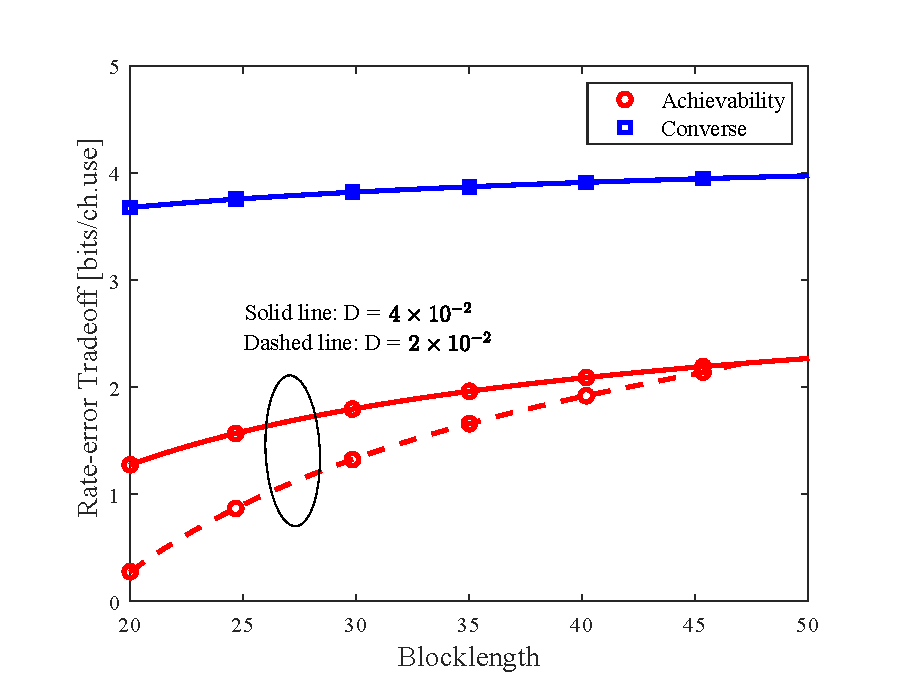
\includegraphics[width = 9cm,height = 7cm]{Fig_rate_error.eps}
    \caption{ The achievability and converse bounds for the rate-error tradeoff with varying code blocklength}
    \label{Fig_rate_error}
\end{figure}


\section{Simulation Results}
In this section, we perform some simulation experiments to consolidate our theoretical bounds and calculate the rate-error region numerically. 

First, we verify the effectiveness of the achievability and converse bounds derived for the rate-error tradeoff $R^\star(N,\epsilon,D)$. Consider the signal model given by \eqref{Channel}, where the per-codeword power budget and the noise variance are set as $\rho = 10$ and $\sigma = 1$, respectively. The channel gain is assumed to belong to the set $|h|\in[1,1.5]$. The achievability and converse bounds of the rate-error tradeoff $R^\star(N,\epsilon,D)$ with varying blocklength $N$ is shown in Fig. \ref{Fig_rate_error}. The probability of decoding error is set to be $\epsilon = 10^{-3}$, while the sensing performance is set to be $D = 4\times10^{-2}\ \mathrm{and}\ 2\times10^{-2}$, respectively. 



According to Fig. \ref{Fig_rate_error}, we find that the converse bounds always outperform the achievability bounds, which is invariant with the sensing performance $D$ since the loss term almost vanishes according to our theoretical analysis. As for the achievability bounds, the rate-error tradeoff increases as $D$ increases since the sensing constraint is relaxed. When $N$ is large enough, the S\&C performance is decoupled, which implies that the two achievability bounds converge to the same value $\tilde{R}^\mathrm{L}_\mathrm{com}(N,\epsilon)$.

Then we calculate the rate-error region $\mathcal{F}(N,\epsilon)$ numerically, which are based on the achievability bound since it can provide a more accurate characterization of the performance tradeoff between S\&C than the converse bound. The system parameters are set the same as above. The achievable rate-error region is shown in Fig. \ref{Fig_region} with the blocklength set to be $N = 20,30,40$, respectively.

\begin{figure}[t]
    \centering
    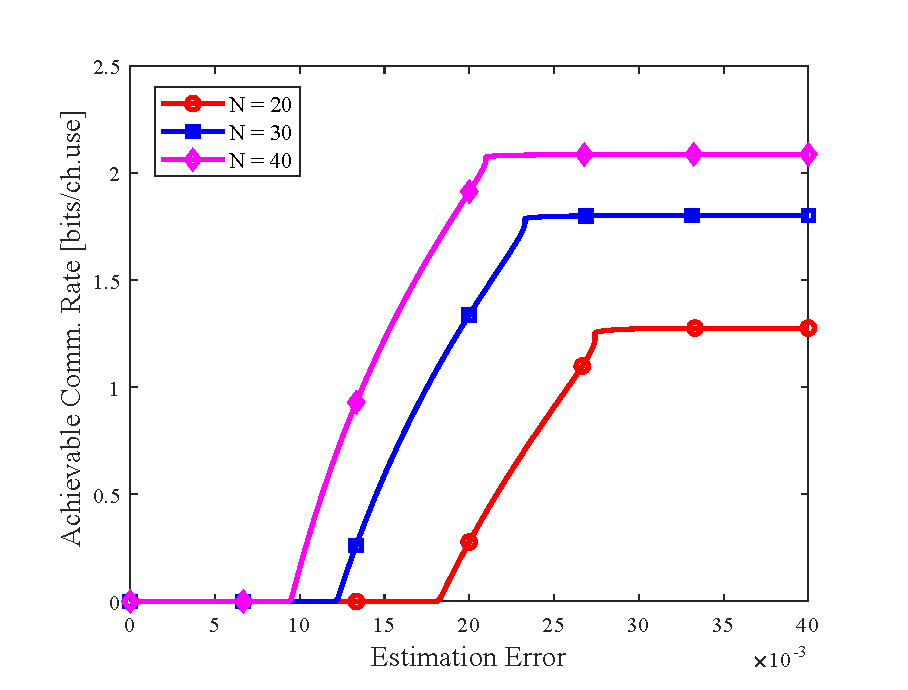
\includegraphics[width = 9cm,height = 7cm]{Fig_region.eps}
    \caption{ The achievable rate-error region with the varying blocklength}
    \label{Fig_region}
\end{figure}


According to Fig. \ref{Fig_region}, we find that as $D$ increases, the achievable rate $R$ remains to be zero at first. When $D$ exceeds the threshold bigger than $\sigma^2/N\rho$, the achievable rate $R$ starts to increase since the achievability bound requires the feasible codeword set $\mathcal{W}$ large enough to carry information. As $D$ moves close to $D_\mathrm{m}$, the coefficient $\gamma_\mathrm{L}$ approaches $1/2$ according to \eqref{Achievability-rate-loss}. However, it switches from $1/2$ to $1$ when $D$ moves past $D_\mathrm{m}$, which leads to the $1/N$ sharp increase in the rate-error tradeoff shown in Fig. \ref{Fig_region}. Then the boundary is invariant of $D$, indicating that the S\&C performance is decoupled.

Furthermore, the area of the rate-error region increases with the blocklength $N$, since the performance tradeoff between S\&C vanishes in the large blocklength regime. As the blocklength $N$ tends to infinity, the boundary of the achievable rate-error region approaches the horizontal line with height $\log_2(1+N\rho|h|_\mathrm{L}^2/\sigma^2) $.
% An example of a floating figure using the graphicx package.
% Note that \label must occur AFTER (or within) \caption.
% For figures, \caption should occur after the \includegraphics.
% Note that IEEEtran v1.7 and later has special internal code that
% is designed to preserve the operation of \label within \caption
% even when the captionsoff option is in effect. However, because
% of issues like this, it may be the safest practice to put all your
% \label just after \caption rather than within \caption{}.
%
% Reminder: the "draftcls" or "draftclsnofoot", not "draft", class
% option should be used if it is desired that the figures are to be
% displayed while in draft mode.
%
%\begin{figure}[!t]
%\centering
%\includegraphics[width=2.5in]{myfigure}
% where an .eps filename suffix will be assumed under latex, 
% and a .pdf suffix will be assumed for pdflatex; or what has been declared
% via \DeclareGraphicsExtensions.
%\caption{Simulation results for the network.}
%\label{fig_sim}
%\end{figure}

% Note that the IEEE typically puts floats only at the top, even when this
% results in a large percentage of a column being occupied by floats.


% An example of a double column floating figure using two subfigures.
% (The subfig.sty package must be loaded for this to work.)
% The subfigure \label commands are set within each subfloat command,
% and the \label for the overall figure must come after \caption.
% \hfil is used as a separator to get equal spacing.
% Watch out that the combined width of all the subfigures on a 
% line do not exceed the text width or a line break will occur.
%
%\begin{figure*}[!t]
%\centering
%\subfloat[Case I]{\includegraphics[width=2.5in]{box}%
%\label{fig_first_case}}
%\hfil
%\subfloat[Case II]{\includegraphics[width=2.5in]{box}%
%\label{fig_second_case}}
%\caption{Simulation results for the network.}
%\label{fig_sim}
%\end{figure*}
%
% Note that often IEEE papers with subfigures do not employ subfigure
% captions (using the optional argument to \subfloat[]), but instead will
% reference/describe all of them (a), (b), etc., within the main caption.
% Be aware that for subfig.sty to generate the (a), (b), etc., subfigure
% labels, the optional argument to \subfloat must be present. If a
% subcaption is not desired, just leave its contents blank,
% e.g., \subfloat[].


% An example of a floating table. Note that, for IEEE style tables, the
% \caption command should come BEFORE the table and, given that table
% captions serve much like titles, are usually capitalized except for words
% such as a, an, and, as, at, but, by, for, in, nor, of, on, or, the, to
% and up, which are usually not capitalized unless they are the first or
% last word of the caption. Table text will default to \footnotesize as
% the IEEE normally uses this smaller font for tables.
% The \label must come after \caption as always.
%
%\begin{table}[!t]
%% increase table row spacing, adjust to taste
%\renewcommand{\arraystretch}{1.3}
% if using array.sty, it might be a good idea to tweak the value of
% \extrarowheight as needed to properly center the text within the cells
%\caption{An Example of a Table}
%\label{table_example}
%\centering
%% Some packages, such as MDW tools, offer better commands for making tables
%% than the plain LaTeX2e tabular which is used here.
%\begin{tabular}{|c||c|}
%\hline
%One & Two\\
%\hline
%Three & Four\\
%\hline
%\end{tabular}
%\end{table}


% Note that the IEEE does not put floats in the very first column
% - or typically anywhere on the first page for that matter. Also,
% in-text middle ("here") positioning is typically not used, but it
% is allowed and encouraged for Computer Society conferences (but
% not Computer Society journals). Most IEEE journals/conferences use
% top floats exclusively. 
% Note that, LaTeX2e, unlike IEEE journals/conferences, places
% footnotes above bottom floats. This can be corrected via the
% \fnbelowfloat command of the stfloats package.
%\section{Acknowledgement}
%This research was supported in part, by Basic Research
%Strengthening Program of China (173 Program) (2020-JCJQZD-015-01), the National Natural Science Foundation of China under Grant 62271285, and National Key R\&D Program of China 2020YFC151180.


\section{Conclusion}
This paper provides a characterization of the performance tradeoff between S\&C in a SISO ISAC system with finite blocklength where the rate-error tradeoff is introduced as the performance metric. In particular, we derive the achievability and converse bounds for the rate-error tradeoff, after which the asymptotic analysis is performed to show that the performance tradeoff vanishes as the blocklength tends to infinity. Finally, our theoretical results are verified by the numerical experiments. Future work will focus on obtaining tighter bounds for the rate-error tradeoff as well as the extension to MIMO ISAC systems. The contributions of this paper give insights to the understanding of the fundamental tradeoff and the future system design in ISAC.



% conference papers do not normally have an appendix


% use section* for acknowledgment


\bibliographystyle{IEEEtran}
\bibliography{IEEEabrv,StringDefinitions,SGroupDefinition,SGroup}


% trigger a \newpage just before the given reference
% number - used to balance the columns on the last page
% adjust value as needed - may need to be readjusted if
% the document is modified later
%\IEEEtriggeratref{8}
% The "triggered" command can be changed if desired:
%\IEEEtriggercmd{\enlargethispage{-5in}}

% references section

% can use a bibliography generated by BibTeX as a .bbl file
% BibTeX documentation can be easily obtained at:
% http://mirror.ctan.org/biblio/bibtex/contrib/doc/
% The IEEEtran BibTeX style support page is at:
% http://www.michaelshell.org/tex/ieeetran/bibtex/
%\bibliographystyle{IEEEtran}
% argument is your BibTeX string definitions and bibliography database(s)
%\bibliography{IEEEabrv,../bib/paper}
%
% <OR> manually copy in the resultant .bbl file
% set second argument of \begin to the number of references
% (used to reserve space for the reference number labels box)




% that's all folks
\end{document}



